\documentclass[12pt]{article}

  \usepackage{geometry}
\geometry{left=0.1in, right=0.1in, top=0.25in, bottom=0in}


\usepackage[inline]{enumitem}
\usepackage{ifthen}


\usepackage{tikz,pgfplots}
\usetikzlibrary{shadows,arrows,positioning,calc, fit}

\makeatletter
\newcommand{\Distance}[3]{% % from https://tex.stackexchange.com/q/56353/121799
\tikz@scan@one@point\pgfutil@firstofone($#1-#2$)\relax  
\pgfmathsetmacro{#3}{veclen(\the\pgf@x,\the\pgf@y)}
}% Explanation: the calc library allows us, among other things, to add and
% subtract points, so ($#1-#2$) is simply the difference between the points
% #1 and #2. The combination \tikz@scan@one@point\pgfutil@firstofone extracts
% the coordinates of the new point and stores them in \pgf@x and \pgf@y. 
% They get fed in veclen, and \pgfmathsetmacro stores the result in #3. 
\makeatother


% Define the layers to draw the diagram
\pgfdeclarelayer{background}
\pgfdeclarelayer{foreground}
\pgfsetlayers{background,main,foreground}

% Define block styles
% \tikzstyle{materia}=[draw, fill=blue!20, text width=6.0em, text centered, minimum height=1.5em,drop shadow]
\tikzstyle{course} = [draw, text centered, minimum width=5em,
  minimum height=2em, rounded corners, drop shadow]
% \tikzstyle{texto} = [above, text width=6em, text centered]
\tikzstyle{linepart} = [draw, very thick, color=magenta!50!black, -latex', dashed]
\tikzstyle{coreq} = [draw, very thick, color=black, -latex', dashed]
\tikzstyle{line} = [draw, very thick, color=magenta!50!black, -latex']
% \tikzstyle{ur}=[draw, text centered, minimum height=0.01em]


\newcommand{\remedial}[3]{node (p#2) [course, minimum width=2em, fill=orange,#1]{#3}}

\newcommand{\alpcourse}[3]{node (p#2) [course, minimum width=2em, fill=brown, #1]{#3}}

\newcommand{\credit}[3]{node (p#2) [course, minimum width=5em, fill=blue!35!white, #1]{#3}}

% Draw background
\newcommand{\background}[4]{%
    % Left-top corner of the background rectangle
    \path (#1.west |- #1.north)+(-0.5,0.5) node (#3-nw) {};
    % Right-bottom corner of the background rectangle
    \path (#1.north -| #2.east)+(0.5,0.5) node (#3-ne) {};
    % Left-lower corner of the background rectangle
    \path (#2.east |- #2.south)+(0.5,-0.5) node (#3-se) {};
    % Right-upper corner of the background rectangle
    \path (#2.south -| #1.west)+(-0.5,-0.5) node (#3-sw) {};
    % Draw the background
    \path[#4]
      (#3-nw) rectangle (#3-se);
    % \coordinate (w) at ($(nw.west)!0.5!(ne.west)$);
    % \coordinate (e) at ($(a3.east)!0.5!(a4.east)$);
    % \coordinate (n) at ($(ne.west)!0.5!(a3.west)$);
    % % \coordinate (s) at ($(nw.east)!0.5!(a4.east)$);
    %   \path[very thick, draw=#4]
    %   (n.north)+(-0.2,0) node[above, text centered, #5]{#6};
    % \ifthenelse{#3=8}
    %        {
    %         \path[very thick, draw=#7]
    %         (n.north)+(0.1,0)--+(0.1,0) node[left, text centered, #6]{#4};
    %        }
    %        { \path[very thick, draw=#7]
    %        (e.east)+(-0.1,0)--+(0.1,0) node[right, text centered, #6]{#4};
    %        }
}




\begin{document}
\pagestyle{empty}

\vspace*{-\baselineskip}
\null\vfill

\centerline{\textbf{\Large Courses Offered by the Math \& CS Department at QCC}}
% \vspace{-0.5\baselineskip}

\begin{center}
\begin{tikzpicture}[scale=0.7,transform shape, font=\Large\sffamily]


\begin{pgfonlayer}{foreground}


  
\begin{scope}[node distance=9.25]
    \path \remedial{minimum height=12.5em,text width=4.0em}{10}{MA-10};
    \path  \remedial{left=of p10.north west, anchor=north, text width=5em}{71}{MA-71};
    \end{scope}
    \begin{scope}[node distance=6.5]
    \path \remedial{right=of p10.north east, anchor=north, text width=8em}{10plus}{MA-10 PLS$^\dagger$};
\end{scope}

\begin{scope}[node distance=6.5]
    \path \alpcourse{left=of p10.south west, anchor=south, minimum height=7.00em, text width=8.5em}{321alp}{MA-321/ MA-321 ALP};
\end{scope}

\begin{scope}[node distance=3.5]
    \path \remedial{right=of p10.south east, anchor=south, minimum height=7.00em, text width=7.1em}{10ws}{MA-10 WS$^\ast$};
\end{scope}


\begin{scope}[node distance=10.5]
    \path \alpcourse{right=of p10.south east, anchor=south, text width=8em}{119alp}{MA-119/ MA-10 ALP};
\end{scope}


\path (p10.south)+(-10,-3.00) \credit{}{321}{MA-321};
\path (p10.south)+(-7,-3.00) \credit{}{301}{MA-301};
\path (p10.south)+(-3,-3.00) \credit{}{100}{CS-100};
\path (p10.south)+(0,-3.00) \credit{}{114}{MA-114};
\path (p10.south)+(3,-3.00) \credit{}{119}{MA-119};
\path (p10.south)+(10,-3.00) \credit{}{121}{MA-121};


%%%%%%%% MA 10 to courses
\coordinate (below10) at ($(p10.south)+(0,-1.750)$);
\coordinate (below10r) at ($(p10.south)+(1,-1.750)$);

\path[draw, very thick, color=magenta!50!black]  (p10.south)--(below10);


%%% 10 to ends: MA121 and 321
\path [line] (below10) -|  ($(p121.north)+(0.0,0)$);
\path [line] (below10) -| ($(p321.north)+(0,0)$);


%%% 10 to 301
\coordinate (above301) at ($(below10)!(p301.north)!(below10r)$);
\path [line] (above301)-- ($(p301.north)+(0,0)$);

%%% 10 to 121
\coordinate (above119) at ($(below10)!(p119.north)!(below10r)$);
\path [line] (above119)--  ($(p119.north)+(0,0)$);

%%% 10 to 114
\coordinate (above114) at ($(below10)!(p114.north)!(below10r)$);
\path [line] (above114)--  ($(p114.north)+(0,0)$);

%%% 10 to 100
\coordinate (above100) at ($(below10)!(p100.north)!(below10r)$);
\path [line] (above100)--  ($(p100.north)+(0,0)$);



%%%%% MA10 Workshop to courses
\coordinate (above10ws) at ($(below10)!(p10ws.south)!(below10r)$);
\path[draw, very thick, color=magenta!50!black]  (p10ws.south)--(above10ws);

\coordinate (above10plus) at ($(below10)!(p10plus.south)!(below10r)$);
\path[draw, very thick, color=magenta!50!black]  (p10plus.south)--(above10plus);

%%%%%% 71 to 321
\coordinate (321w) at (p71|-p321.north);
\path [line,color=red!45!black] (p71.south)+(-0.0,0)-- (321w);



\path (p114.south)+(0,-4.25) \credit{}{128}{MA-128};
\path (p100.south)+(0,-4.25) \credit{}{336}{MA-336};
\path (p119.south)+(0,-4.25) \credit{}{440}{MA-440};
\path (p301.south)+(-1.5,-4.25) \credit{}{303}{MA-303};






% only114

\path [line, color=green!50!black] (p114.south) -- ($(p128.north)+(-0.0,0)$);
\path [line, color=green!50!black] (p114.south)-- ($(p336.north)+(0.6,0)$);
\path [line, color=green!50!black] (p114.south)-- ($(p440.north)+(-0.6,0)$);

% 119+121
\path [coreq] (p119)-- (p121) node [above, midway,font=\Large] {co-requisite};

\coordinate (119-121) at  ($(p119.south)!0.5!(p121.south)$);

\path [draw, very thick, color=red, semithick, double, double distance=1.5pt] (p119.south)+(0.6,0)--+(0.6,-0.5) -|
($(p121.south)+(-0.6,0)$);  %%%% connect 119+121



%% 119+121 to 128
\path [line, color=red, semithick, double, double distance=1.5pt] (119-121)+(0,-0.5)--+(0,-3.00)-| ($(p128.north)+(0.6,0)$); 

%% 119+121 to 440
\coordinate (above440) at  ($(p119.south)+(0,-3.00)$);
\path [line, color=red, semithick, double, double distance=1.5pt] (above440)--(p440.north); 



%%% 119ALP join 121 and then join with 119-121

\coordinate (below121) at ($(p121.south)+(0.6,-0.5)$);
\coordinate (below119alp) at (below121-| p119alp.south);
\coordinate (119alp-121) at  ($(below121)!0.5!(below119alp)$);

\path [draw, very thick, color=red, semithick, double, double distance=1.5pt] ($(p121.south)+(0.6,0)$)--+(0.0,-0.5) -| (p119alp.south);

\path [draw, very thick, color=red, semithick, double, double distance=1.5pt] ($(119-121)+(0.0,-1.250)$)-| (119alp-121);


% only 119

%%% 119 to 303
\path [line,, color=blue!75] (p119.south)+(-0.0,0)--+(-0.0,-2.50)-|($(p303.north)+(0,0)$); 

%%% 119 to 336
\coordinate (below119a) at  ($(p119.south)+(-0.6,-2.50)$);
\coordinate (below119b) at  ($(p119.south)+(0.6,-2.50)$);
\coordinate (above336) at  ($(below119a)!(p336.north)!(below119b)$);

\path [line, color=blue!75] ($(above336)+(0,0)$) -- ($(p336.north)+(0,0)$);



% only 119ALP
%%% 119ALP join 119
\path [draw, very thick, color=blue!75] ($(p119alp.south)+(0.6,0)$)|-($(p119.south)+(-0.6,-2.50)$); %%% 





%%%%%% Sequential courses to 440.

\path (p440.south)+(-7.5,-3.25) \credit{}{441}{MA-441};

\path (p441)+(9, 0.0) \credit{}{101}{CS-101};

\path (p440.south)+(-13,-3.25) \credit{}{471}{MA-471};

\path (p441)+(16,0.0) \credit{}{905}{MA-905};

\path (p441.south)+(-1.75,-3.0) \credit{}{442}{MA-442};
\path (p441.south)+(1.75,-3.0) \credit{}{461}{MA-461};
\path (p471.south)+(0,-3.0) \credit{}{220}{CS-220};


\path (p442.south)+(-3.75,-3.0) \credit{}{443}{MA-443};
\path (p442.south)+(10.75,-3.0) \credit{}{481}{MA-481};

\path (p442.south)+(3.75,-3.0) \credit{}{451}{MA-451};

\path (p905.south)+(0,-3.0) \credit{}{906}{MA-906};

\path (p101.south)+(-3,-3.0) \credit{}{201}{CS-201};
\path (p101.south)+(0,-3.0) \credit{}{203}{CS-203};
\path (p101.south)+(3,-3.0) \credit{}{204}{CS-204};


%%%%% 440 to other courses
\coordinate (below440) at ($(p440.south)+(0,-2.0)$);
\path [line]  (p440.south)--(below440)-|(p471.north);

\coordinate (above441) at (below440-|p441);
\path [line] (above441)--(p441.north);

\path [line] (below440) -|  (p905.north);



%%%%% 441 to other courses

\path [line] (p441.south) --  (p442.north);
\path [line] (p441.south) --  (p461.north);
% \path [coreq] (p441.east) -| (p101.north) node [above, midway, xshift=-3.75cm] {co-requisite};
\path [coreq] (p441.east) -- (p101.west) node [above, midway, font=\Large] {co-requisite};
\path [line] (p471.south) --  (p220.north);
\path [line] (p905.south) --  (p906.north);



\path [line] (p101.south) -- (p201.north);
\path [line] (p101.south)-- (p203.north);
\path [line] (p101.south)-- (p204.north);

\path [line] (p442.south) --  (p443.north);
\path [line] (p442.south) --  (p451.north);
\path [line] (p442.south) --  (p481.north);

\path [coreq] (p443.east) --  (p451.west) node [above, midway, font=\Large] {co-requisite};

\end{pgfonlayer}






%%%%%% Quantitative way

\path (p71.north west)+(-1, 0.25) node (qw-nw) {};
\path (p119alp.east)+(1,-23) node (lower-right) {};

\coordinate (QuantLRCorner) at ($(p303)+(3, -0.75)$);



\begin{pgfonlayer}{main}
\background{qw-nw}{QuantLRCorner}{quant}{fill=green!15};
\coordinate (quant-n) at ($(quant-nw.west)!0.5!(quant-ne.east)$);
    % \coordinate (s) at ($(nw.east)!0.5!(a4.east)$);
\path (quant-n)+(0,-0.125) 
let \p1 = ($ (quant-nw)-(quant-ne) $),
\n{stemwidth} = {veclen(\x1,\y1)}
in
node[above, text centered, minimum width=\n{stemwidth}, minimum height=3em,fill=green!15] (nodequant) {\textbf{\Large NON-STEM}};
\end{pgfonlayer}

\begin{pgfonlayer}{background}

\background{qw-nw}{lower-right}{path}{fill=lime!25};
\coordinate (path-n) at ($(path-ne.east)!0.5!(quant-ne.west)$);
    % \coordinate (s) at ($(nw.east)!0.5!(a4.east)$);
\path (path-n)+(0,-0.125) 
let \p1 = ($ (path-ne)-(quant-ne) $),
\n{pathwidth} = {veclen(\x1,\y1)}
in
node[above, text centered, minimum width=\n{pathwidth}, minimum height=3em, fill=lime!25] (nodepath) {\textbf{\Large STEM}};
\end{pgfonlayer}



%%%%%%%%%%%% Placement Exam node

\begin{pgfonlayer}{foreground}

    \coordinate (ACCFiveT) at (path-nw.north);
    \coordinate (ACCFiveBy) at ($(p321alp.south)+(0, -3.00)$);
    \coordinate (ACCFiveB) at (path-nw.north|-ACCFiveBy);

\Distance{(ACCFiveT)}{(ACCFiveB)}{\ACCFive}

\coordinate (ACCMath5L) at ($(nodequant.north west)+(0.15,0)$);
\coordinate (ACCMath5R) at ($(nodepath.north east)+(0,0)$);

\path  (ACCMath5L) node[below left, text centered, minimum width=3em, minimum height=\ACCFive, fill=cyan!50]  {\rotatebox{90}{\Huge ACCMath5 \qquad Score}};

\path  (ACCMath5R) node[below right, text centered, minimum width=3em, minimum height=\ACCFive, fill=cyan!50]  {\rotatebox{90}{\Huge ACCMath5 \qquad Score}};

\coordinate  (ACCMath6L) at ($(ACCMath5L)+(-1.5em, -0.0\textwidth)$);
\path (ACCMath6L)  node[below, anchor=north, text centered, minimum width=3em, minimum height=0.35\textheight,fill=cyan!75, yshift=-\ACCFive]{\rotatebox{90}{\Huge ACCMath6 \qquad Score}};

\coordinate  (ACCMath6R) at ($(ACCMath5R)+(1.5em, -0.0\textwidth)$);
% \coordinate  (ACCMath6R) at (ACCMath5R|-ACCFiveB);

\path (ACCMath6R)  node[below, anchor=north,yshift=-\ACCFive, text centered, minimum width=3em, minimum height=0.35\textheight,fill=cyan!75]{\rotatebox{90}{\Huge ACCMath6 \qquad Score}};


%%%%% Placement to 321alp


\coordinate (Sp71) at ($(p71.south)+(0,-0.75)$);

\coordinate (ACCp71L) at (ACCMath5L.west|-Sp71);

\coordinate (R321Alp) at ($(p321alp)!0.5!(p321alp-|quant-ne)$);
% \coordinate (ACCp71R) at ($(p71.east|-Sp71)+(3,0)$);
\coordinate (ACCp71R) at (R321Alp|-Sp71);

\path[line width=0.2pt, dashed, draw=cyan!50] (ACCp71L)-- (ACCp71R);

\node[above right, xshift=-0.25pt, fill=cyan!50] at (ACCp71L) {\rotatebox{90}{below 40}};
% \node[above left, xshift=-0.25pt, fill=cyan!50] at ($(ACCp71R)-(0.75,0)$) {\rotatebox{90}{below 40}};

% \node[below left, xshift=-0.25pt, fill=cyan!50] at ($(ACCp71R)$) {\rotatebox{-90}{40 or higher}};

\coordinate (Sp10plus) at ($(p10plus.south)+(0,-0.75)$);

\coordinate (ACCp10plusR) at (ACCMath5R.east|-Sp10plus);

\coordinate (MidWS) at ($(p10ws.west)!0.5!(p10.east)$);

\coordinate (ACCp10plusL) at (MidWS|-Sp10plus);

\path[line width=0.2pt, dashed, draw=cyan!50] (ACCp10plusL)-- (ACCp10plusR);

% \node[above right, xshift=-0.25pt, fill=cyan!50] at ($(ACCp10plusL)+(1.5,0)$) {\rotatebox{90}{below 40}};

\node[above left, xshift=0.25pt, fill=cyan!50] at (ACCp10plusR) {\rotatebox{90}{below 40}};

% \node[below, fill=cyan!50] at (ACCp10plusL) {\rotatebox{-90}{40 or higher}};

%%%%% Placement to 119alp (47-56)

\coordinate (Sp119alpT) at ($(p119alp.north)+(0,0.75)$);

\coordinate (ACCp119alpTR) at (ACCMath5R.west|-Sp119alpT);

\coordinate (ACCp119alpTL) at ($(p119alp.west|-Sp119alpT)+(-1,0)$);

\path[line width=0.2pt, dashed, draw=cyan!50] (ACCp119alpTL)-- (ACCp119alpTR) node[left, fill=cyan!50] {47};
% \node[below left, xshift=0.25pt, fill=cyan!50] at (ACCp119alpTL) {\rotatebox{-90}{47 or higher}};


%%%%% Placement to 321alp and 10alp (below 57)

\coordinate (Sp10B) at ($(p10.south)+(0,-0.75)$);

\coordinate (ACCp10BL) at (ACCMath5L.west|-Sp10B);

\coordinate (ACCp10BR) at (ACCMath5R.east|-Sp10B);

\path[line width=0.2pt, dashed, draw=cyan!50] (ACCp10BL)-- (ACCp10BR);
\node[above right, xshift=-0.25pt, fill=cyan!50] (scoreCL) at (ACCp10BL) {\rotatebox{90}{below 57}};
\node[above left, xshift=0.25pt, fill=cyan!50] (scoreCR) at (ACCp10BR) {\rotatebox{90}{below 57}};
% \node[below right, xshift=-0.25pt, fill=cyan!50] at (scoreCL.south east) {\rotatebox{-90}{57 or higher}};
% \node[below left, xshift=0.25pt, fill=cyan!50] at (scoreCR.south west) {\rotatebox{-90}{57 or higher}};





%%%%% Placement to 440

\coordinate (Sp119) at ($(p119.south)+(0,-1.750)$);

\coordinate (ACCp119L) at (ACCMath5L.west|-Sp119);

\coordinate (ACCp119R) at (ACCMath5R.east|-Sp119);

\path[line width=0.2pt, dashed, draw=cyan!75] (ACCp119L)-- (ACCp119R);
\node[above right, xshift=-0.25pt, fill=cyan!75] (scoreBL) at (ACCp119L) {\rotatebox{90}{below 60}};

\node[above left, xshift=0.25pt, fill=cyan!75] (scoreBR) at (ACCp119R) {\rotatebox{90}{below 60}};

% \node[below right, xshift=-0.25pt, fill=cyan!75] at (scoreBL.south east) {\rotatebox{-90}{60 or higher}};
% \node[below left, xshift=-0.25pt, fill=cyan!75] at (scoreBR.south west) {\rotatebox{-90}{60 or higher}};


%%%%% Placement to 441

\coordinate (Sp440) at ($(p440.south)+(0,-1.0)$);

\coordinate (ACCp440L) at (ACCMath5L.west|-Sp440);

\coordinate (ACCp440R) at (ACCMath5R.east|-Sp440);

\path[line width=0.2pt, dashed, draw=cyan!75] (ACCp440L)-- (ACCp440R);
\node[above right, xshift=-0.25pt, fill=cyan!75] (scoreAL) at (ACCp440L) {\rotatebox{90}{below 80}};
\node[above left, xshift=0.25pt, fill=cyan!75] (scoreAR) at (ACCp440R) {\rotatebox{90}{below 80}};
% \node[below right, xshift=-0.25pt, fill=cyan!75] at (scoreAL.south east) {\rotatebox{-90}{80 or higher}};
% \node[below left, xshift=-0.25pt, fill=cyan!75] at (scoreAR.south west) {\rotatebox{-90}{80 or higher}};


\end{pgfonlayer}


%%%%% Remarks on courses

\coordinate (rmk-1) at ($(path-nw)+(0,0.5)$);
\coordinate (path-ne-west) at ($(path-ne)+(0,0)$);
\coordinate (path-nw-east) at ($(path-nw)+(0,0)$);
\Distance{(path-nw-east)}{(path-ne-west)}{\picwidth}

\node[above=of rmk-1, anchor=west, fill=blue!35!white, yshift=5pt, minimum width={\picwidth}] (rmk-cre) {Other courses are credit-bearing courses.};
\node[above=of rmk-cre.west, anchor=west, fill=brown, yshift=-5.5pt, minimum width={\picwidth}] (rmk-hyb) {Courses in brown color are remedial and credit-bearing linked courses.};
\node[above=of rmk-hyb.west, anchor=west, fill=orange, yshift=-4.5pt, minimum width={\picwidth}] (rmk-rem) {Courses in orange color are remedial/non-credit courses.};

\end{tikzpicture}

\parbox{0.915\textwidth}
{
\it
 % \vspace{-\baselineskip}
    \scriptsize 
    % \small 

    $\ast$: \begin{enumerate*}[label={(\roman*)}]
        \item multiple repeaters of MA 10 (i.e. failed MA 10 two or more times), and 
        \item first-time repeaters of MA 10 or MA-10 ALP with score of at least 40 on the CEAFE %may also be enrolled in MA-10 WS.
        % \item repeaters with a score at least 40 on the CEAFE or 
        % \item students with a R grades for MA-10 ALP and a score at least 40 on the CEAFE
    \end{enumerate*}
    may also be enrolled in MA-10 WS.

$\dagger$: 
First-time repeaters of MA 10 or MA-10 ALP with score of 39 or below on the CEAFE may also be enrolled in MA-10 PLS. 
% \begin{enumerate*}[label={(\arabic*)}]
%     \item Repeaters with a score 39 or below on the CEAFE or
%     \item students with a R grades for MA-10 ALP and a score 39 or below on the CEAFE
% \end{enumerate*} 
% may also be enrolled in MA-10 WS.

   
}
\end{center}


\vfill\null
\end{document}